\documentclass[USenglish]{article}

\usepackage{ifikompendiumforside}
\usepackage{graphicx}
\usepackage[acronym]{glossaries}
\usepackage[backend=biber,sorting=none]{biblatex}

\makeglossaries

% Acronyms
\newacronym{dil}{DIL}{Disconnected, Intermittent and Limited environments}

\title{Improving the performance of Web Services in Disconnected, Intermittent and Limited Environments}
\author{Joakim Johanson Lindquister}
\bibliography{references}

\begin{document}
\ififorside{}

\begin{abstract}
    My abstract
\end{abstract}
\pagebreak

\tableofcontents
\listoftables
\listoffigures

\pagebreak


\part{Introduction}
Kort intro om oppgaven her.
\section{Background and Motivation}
\subsection{Mobile tactical networks}
Mobile tactical networks are characterized by that the units use tactical
communication equipment which includes technologies like VHF, UHF, HF, tactical
broadband and satellites. Examples of such units are mobile units like vehicles,
foot soldiers and field headquarters. These types of networks have low
bandwidth, possibly high delay, high error rates and frequent disconnections.
They are often called disadvantaged grids or DIL. NATO studies has
identified such networks to have the following characteristics:

\paragraph{}
\textit{Disadvantaged grids are characterized by low bandwidth, variable
throughput, unreliable connectivity, and energy constraints imposed by the
wireless communications grid that link the
nodes}\cite{nato-disadvantaged-grids}.

\paragraph{}
These constrains of mobile tactical networks are central in order to understand the problem at hand, and I will therefore explain the concepts here:

\begin{description}
\item[Bandwidth and throughput] The terms bandwidth and throughput are used interchangeably in the networking community and refers to the data transfer rate; how fast data can be transported from one point to another in given time period. This is often expressed in bits per second.
\item[Unreliable connectivity] Units that are participating in a tactical network are highly mobile and may disconnect from a network either voluntarily or not. Unplanned loss of connectivity can be due to various reasons, such as loss of signal or equipment malfunction.
\item[Energy constraints imposed by the wireless communication grid] The battery capacity and the transmission range of the communication equipment for mobile units may be limited. Another issue is that in some cases military units are required to enter radio silence in order to avoid being detected by the enemy. During radio silence units may only receive data and not send any.
\end{description}

\section{Problem Statement}
Most of the Web Service solutions used today are aimed for civilian use and does
not necessarily perform well in military environments. In contrast to civilian
networks where bandwidth are abundant, mobile tactical networks may suffer
from high error rates and low bandwidth.

In my master thesis I will investigate different optimization techniques that
can be applied to improve communication. In order for the clients and services
 to remain interoperable the optimization techniques will be placed in proxies.

The Web Services will communicate with his counter part over HTTP as regular,
with all traffic going umerkelig through the proxy. The Web Service itself does
not need to pay attention to the bad connectivity, the proxy will choose the
appropriate protocol and configuration.

\section{Premises}
Ikke endre web-servicene.

\section{Scope and Limitations}
Snevre inn oppgaven

\section{Research Methodology}

\section{Contribution}
Hva er det oppgaven min bidrar med?
\section{Outline}
Hvordan er resten av oppgaven strukturert.


%%%%% BACKGROUND %%%%
\part{Background}
In this part, I will present relevant technologies.
\section{Related Work}
Diskuterer eksisterende arbeid.
\section{DIL}
\gls{dil} definer hva DIL er og hvilke begrensninger det legger.

\section{Requirement Analysis}
Diskutere CPU-bruk vs compression.
\\ \\ \\
\begin{table}
\begin{tabular}{| l | l |}
\hline
  \textbf{Requirement} & \textbf{Priority} \\ \hline
  Receive and forward HTTP 1.X requests & 1\\ \hline
  Allow modifications on the payload & 1 \\ \hline
  Allow configuration of HTTP timeouts & 1 \\ \hline
  asd & 1 \\ \hline
  Support protocol X and y & 2 \\ \hline
\end{tabular}
\caption{Proxy requirements}
\end{table}

\section{Summary}



%%%% Design and implementation %%%%
\part{Design and Implementation}
\section{Overall Design}
\section{Proxy}
\subsection{Squid}
Squid is a fully-featured HTTP/1.0 proxy.
\begin{figure}[h]
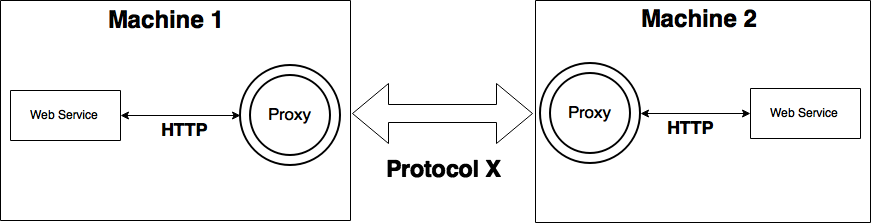
\includegraphics[scale=0.4]{images/architecture.png}
\caption{Architectural overview of proposed design}
\end{figure}

\section{Optimization techniques}
By using proxies, we can freely choose the communcations protocols and
configurations between the proxy pair without altering the Web Services themself.
In this thesis I will investigate different techniques in order to optimize the
communcation between a Web Service and a Web Service client. The first technique
I will look into is compression.

\subsection{Compressing the payload}
Compress the payload using GZIP and forward it to the other proxy. The

\subsection{Tuning application server configuration}

\subsection{Alternative transport protocols}

\section{Summary}

\part{Testing and Evaluation}
\section{Evaluation Tools}

\part{Conclusion and Future Work}
\section{Conclusion}

\section{Future Work}

\pagebreak
\printbibliography{}
\printglossary

\end{document}
